\section{Self-Encoding Structure}
\label{sec:self-encoding}

This section describes how the logic that interprets data is stored in the same verifiable structure as the data itself, using the substrate of \cref{sec:integrity-state} and the history of \cref{sec:history-entanglement}. Data and its interpretation can therefore be retained, transferred, and verified together.

\subsection{Code at Web Scale}

A durable network must survive software change as well as storage failure. Data written today may be read by another organization years later, after schemas, libraries, runtimes, and deployment practices have moved on. Preserving bytes answers only the first half of the archival question, because the reader also needs an account of how those bytes were structured and what operations gave them meaning. The Web already offers several partial approaches. JavaScript carries behavior to a widely available runtime, and Protocol Buffers and similar schema-driven encodings define stable wire forms and evolution rules whose schemas supply interpretation beyond each payload. Package managers and containers capture dependencies, while reproducible-build and software-transparency systems make artifacts traceable to declared sources and environments~\cite{Nikitin2017chainiac}. Each binds a different portion of the path from stored bits to behavior, but the data rarely carries that whole path. The gap matters because, at Web scale, change management crosses administrative boundaries. A recipient may accept data while declining the producer's newest software, or retain an old \glslink{object}{object} long after its originating service has migrated. Reproducibility also demands explicit treatment of time, randomness, network responses, and operator choices. \glslink{self-encoding}{Self-encoding} structure answers these pressures by placing a changeable definition inside the same commitment as the state it interprets. The resulting historical pair can travel, be sliced, and be cited together. The runtime consequently shrinks to a smaller shared foundation, application semantics become versioned material, and transitions can expose the environmental inputs on which their results depend.

\subsection{Lisp as Durable Structure}
\label{sec:lisp-structure}

Lisp gives code and data one inspectable representation. A method definition, query, path, transition, or configuration is an ordinary expression, so the network can hash, store, and transmit it like data and still evaluate it as code. This property, homoiconicity, is the reason for the choice of language. It turns semantic bootstrapping into structural composition, because the network can preserve the form describing an operation with the same substrate that preserves its inputs. The implemented runtime uses s7 Scheme~\cite{Schottstaedt2024s7} inside the \glslink{journal}{journal}. Native primitives provide the substrate of \cref{sec:integrity-state}, namely construction, hashing, persistence, \glslink{slice}{slicing}, network preparation, and controlled evaluation. Everything else, including maps, chains, signed histories, \glslink{authorization}{authorization}, and object protocols, is ordinary Scheme built above them. Because these structures are ordinary programs over the same primitives, applications can define others that favor different performance objectives, such as append-only commitments that give recently added items shorter membership proofs~\cite{Cevallos2025merkle}. The approach follows the tier-unifying intuition of single-language Web systems~\cite{Cooper2007links}, preserving explicit boundaries while reducing translations between stored state and application logic. The bootstrap terminates in native storage and evaluator semantics, which define how expressions are read, \glslink{node}{nodes} are hashed, and capabilities are exposed. Keeping this foundation small makes it practical to inspect and reproduce, and every higher layer can evolve as identified structure in journal history.

Within one language, objects may implement different methods and evolve under different authorities, yet remain transportable through the same node and evaluator model. Documented public behavior provides compatibility across class systems. Confinement is necessary because portable definitions arrive from parties who may use different software and policy. The implemented \texttt{sync-let} boundary copies inputs as plain data into a reduced environment of approved primitives, excludes direct access to the journal, network, time, randomness, and host, and copies results back to the caller as plain data. Finer per-object capability assignment is an optional extension that portable execution does not require. Capability confinement and evaluator isolation address different failures, continuing the distinction between restricted execution environments and other approaches to program safety such as proof-carrying code~\cite{Levy1995safe,Necula1997proof} and object-capability systems~\cite{LemmerWebber2025spritely}. While the evaluator isolates shared computation from host authority, the trusted host still controls persistence, networking, and consumption of compute and storage. Preserving an executable definition does not remove this dependency, because interpreting it still requires compatible evaluator semantics and a trusted execution boundary.

\subsection{Self-Encoding Objects}
\label{sec:objects}

A standard object is a node with executable definition on the left and state on the right. Its \glslink{digest}{digest} commits to both components and to their association. Evaluating that node with \texttt{sync-eval} produces a transient callable object. A zero-argument call returns its current node, documented method dispatch exposes behavior, and object-specific \glslink{path}{paths} expose state according to the object's protocol. \Cref{fig:self-encoding-transition} follows one transition as definition $D_0$ and state $S_0$ enter a controlled runtime with explicit input arguments, producing a candidate with revised definition $D_1$ and \glslink{successor}{successor} state $S_1$. However, evaluation alone changes nothing durable, since an authorized boundary chooses whether to persist that result. Because the starting object remains independently identifiable, semantic change takes the form of historical succession instead of replacement.

\begin{figure}[htbp]
  \centering
  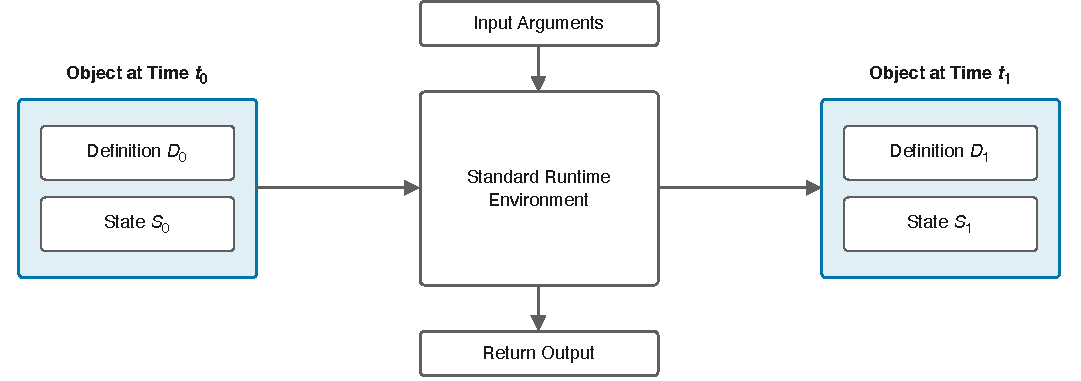
\includegraphics[scale=0.851]{figures/self-encoding-transition.pdf}
  \caption{Self-Encoding Object Transition}
  \label{fig:self-encoding-transition}
\end{figure}

Live and durable mutation are deliberately separate and meet only at explicit persistence. A method may update the live object's state, but the change becomes history only when the journal extracts the new node and stores it into its parent or root. Nested mutation follows the same rule along the return path, where each containing object is rebuilt in turn, every predecessor remains available by digest, and the durable boundary stays visible in code. Objects compose through public protocols, so deep reads can traverse semantic boundaries while deep mutations rebuild ancestors. Deep slicing and \glslink{prune}{pruning} ask each object to retain evidence appropriate to its layout, and deep \glslink{merge}{merge} restores compatible partial material under matching commitments. \Cref{tab:deep-operations} summarizes this implemented family. The caller places shared computation inside the confinement boundary of \cref{sec:lisp-structure} before loading an object with \texttt{sync-eval}, so environmental values reach untrusted code only as copied data. Authorization and storage then turn the candidate result into history.

\begin{table}[htbp]
  \centering
  \small
  \begin{tabularx}{\textwidth}{@{}>{\ttfamily\frenchspacing}P{0.125\textwidth}>{\ttfamily\frenchspacing}P{0.38\textwidth}X@{}}
\toprule
\normalfont\textbf{Operation} & \normalfont\textbf{Signature} & \textbf{Behavior} \\
\midrule
deep-get    & (deep-get object path) & Traverse nested public \texttt{get} methods and return the value at the path. \\
deep-set!   & (deep-set! object path value) & Set the terminal value and rebuild each ancestor. \\
deep-slice! & (deep-slice! object path) & Retain evidence along the path while preserving the logical digest. \\
deep-prune! & (deep-prune! object path) & Remove path evidence, rebuilding parents or replacing exhausted children with stumps. \\
deep-merge! & (deep-merge! source target path) & Merge digest-compatible evidence into the target or into the optional target path. \\
deep-copy!  & (deep-copy! object source target) & Copy the value at one nested path to another. \\
deep-call   & (deep-call object path callback) & Evaluate a callback against the selected object and return its result, leaving ancestors unchanged. \\
deep-call!  & (deep-call! object path callback) & Evaluate once and return the result with the complete rebuilt root. \\
\bottomrule
\end{tabularx}

  \caption{Deep Object Operations}
  \label{tab:deep-operations}
\end{table}

\subsection{Shared Computation in Practice}
\label{sec:shared-computation}

Beyond individual objects, the journal supports several forms of shared computation. The standard object library grows semantics from a small evaluator. Portable classes compose through public protocols, journals place results into signed history, and application-defined objects carry domain concepts. Stored programs use a journal capability to compose standard journal operations, including historical resolution and retention, in the native path, history, and object vocabulary.\footnote{An administrator may also configure one stored program to launch after each successful commit, receiving that commit's index. The launch is best-effort and periodic, since launches may overlap and a process failure after commit can lose a launch.} Historical \texttt{retrieve} can also exercise an object method without persisting its successor. The requesting journal checks the returned proof against the selected commitment and recomputes the result using the definition and state in the proof. These facilities extend the substrate under three controls:

\begin{itemize}[nosep]
  \item \textbf{Deterministic object evaluation.} A confined object's candidate successor derives from its definition, starting state, explicit arguments, compatible evaluator semantics, and controlled primitives. Multi-call stored programs may observe changing journal state and are therefore not fully replayable.
  \item \textbf{Resource governance.} Execution bounds constrain a single operation and its descendants, but aggregate resource exhaustion still requires host-level admission control. Failure discards an uncommitted candidate but does not undo previously completed nested journal operations.
  \item \textbf{Explicit evolution.} Public protocols and layouts are compatibility contracts. Migrations must state authority, validation, rollback, partial-object behavior, and runtime compatibility rather than treating executable history as automatic semantic compatibility.
\end{itemize}

These controls together keep shared computation reproducible where it matters and leave its operational limits to host policy.